\chapter{Ogólny opis systemu}
\label{cha:wprowadzenie}


\section{Cel (przeznaczenie) systemu}
\label{sec:celePracy}

Celem systemu automatyczny parking jest umożliwienie komputerowej obsługi pobierania opłat za~pozostawienie pojazdu na parkingu na określony czas. System rozpoznaje ze zdjęcia tablice rejestracyjne pojazdów i na tej podstawie umożliwia wjazd samochodów na parking, a także opuszczenie go.

\section{Udziałowcy i użytkownicy}

\begin{list}{$\bullet$}{}
\item Właściciel - posiada parking, jest kierownikiem zarządzającym pracownikami, system prezentuje mu zebrane statystki
\item Klient - osoba, która korzysta z usług automatycznego parkingu i wjeżdza samochodem na jego teren
\item Operator - osoba kontrolująca parking w danej chwili, w przypadku błędów, przegląda zarejestrowane zdjęcia i poprawia czas wjazdu/wyjazdu, wprowadza rejestrację pojazdu do systemu oraz w~wyjątkowych sytuacjach podnosi/opuszcza szlaban

\end{list}

\section{Podstawowe cele udziałowców i użytkowników}

\begin{table}[H]
	\begin{tabular}{|l|l|l|} \hline
	\textbf{Udziałowcy}	& \textbf{Cel} & \textbf{Priorytet} \\ \hline% \bottomrule
	Klient	& Wjechanie na parking & Wysoki \\
	Klient	& Opuszczenie parkingu & Wysoki \\
	Klient	& Wpisanie numeru rejestracyjnego & Wysoki \\
	Klient	& Potwierdzenie zdjęcia & Wysoki \\
	Klient	& Anulowanie wpisanego numeru rejestracyjnego & Średni \\
	Klient	& Uiszczenie opłaty & Wysoki \\
	Operator& Przeglądanie zdjęć & Średni \\
	Operator& Wprowadzenie rejestracji & Średni \\
	Operator& Poprawa czasu wjazdu i wyjazdu w bazie & Średni \\
	Operator& Podnoszenie/opuszczanie szlabanu & Średni \\
	Właściciel& Wyświetlenie statystyk & Niski \\ \hline
	\end{tabular}
\end{table}

\subsection{Porównanie proponowanego systemu do aktualnie funkcjonującego}
%płatność kartą i gotówką?
Na parkingu znajdującym się koło Wawelu w Krakowie klient podjeżdża do terminala, naciska przycisk i~odbiera bilet z godziną wjazdu. Przy opuszczaniu parkingu wkłada otrzymany przy wjeździe bilet i~dokonuje opłaty.
W~naszym systemie klient, wjeżdżając na parking, nie musi podjeżdżać do terminala i~czekać na wydrukowanie kartki z~godziną wjazdu. System zrobi zdjęcie tablicy rejestracyjnej i~sam otworzy szlaban. W~ten sposób oszczędzany jest papier oraz tusz. Operator nie musi dbać o~to żeby ich nie zabrakło. Musi jedynie interweniować w~przypadku błędu.


\section{Granice systemu}
\begin{figure}[H]
	\centering
	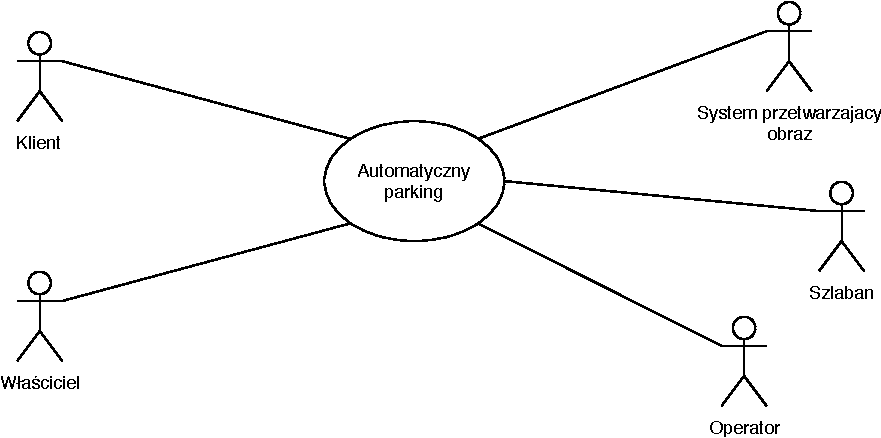
\includegraphics[width=90mm]{diagramy/graniceSystemu.pdf}
	\caption{Granice systemu automatyczny parking }
\end{figure}

\section{Lista funkcji systemu}


\begin{enumerate}
	\item Wykrycie pojawienia się pojazdu
	\item Zapis zdjęcia rejestracji
	\item Zapis tablicy rejestracyjnej
	\item Otwarcie szlabanu
	\item Zamknięcie szlabanu
	\item Wyświetlenie zdjęcia tablicy rejestracyjnej
	\item Obliczenie kwoty do zapłaty
	\item Wyświetlenie kwoty do zapłaty
	\item Oczekiwanie na pojazd do 15 minut
	\item Zgłoszenie niezgodności wpisanej i zarejestrowanej rejestracji
	\item Wyświetlenie wpisanego przez klienta numeru rejestracyjnego
	\item Zapis danych
	\item Prezentacja statystyk
\end{enumerate}

\section{Diagramy czynności}

% Diagram czynności: Klient wjeżdża na parking
\begin{figure}[H]
	\centering
	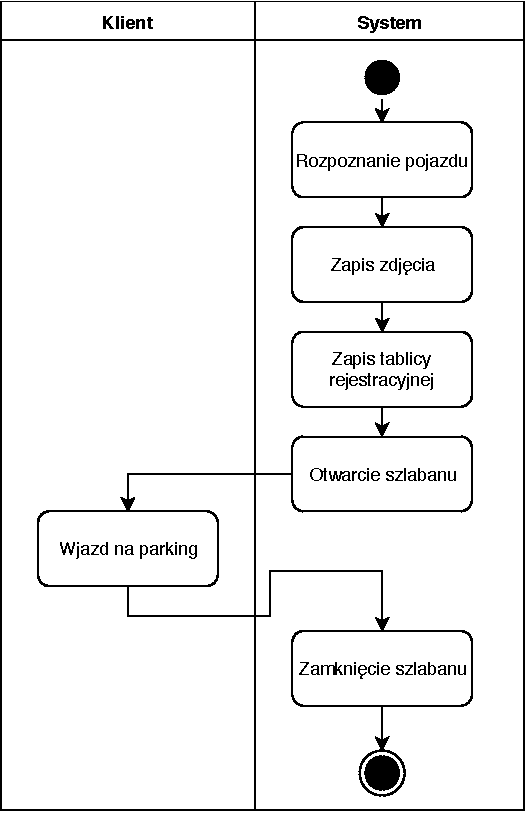
\includegraphics[width=90mm]{diagramy/DiagCzynWjazd.pdf}
	\caption{Diagram czynności: Klient wjeżdża na parking}
\end{figure}


% Diagram czynności: Klient opuszcza parking
\begin{figure}[H]
	\centering
	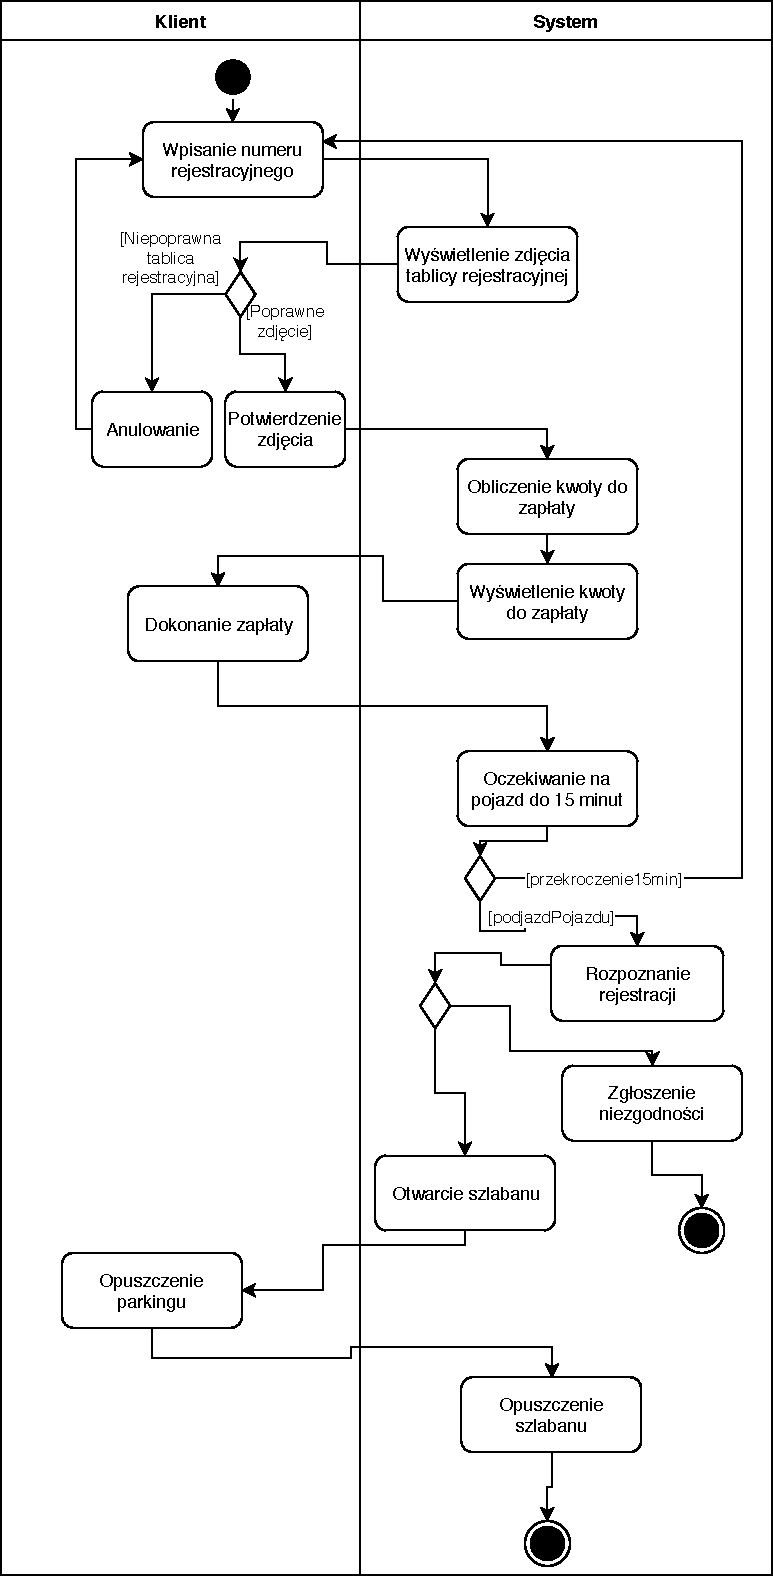
\includegraphics[width=90mm]{diagramy/DiagCzynWyjazd.pdf}
	\caption{Diagram czynności: Klient opuszcza parking}
\end{figure}


% Diagram czynności: Operator weryfikuje wykryte oszustwo
\begin{figure}[H]
	\centering
	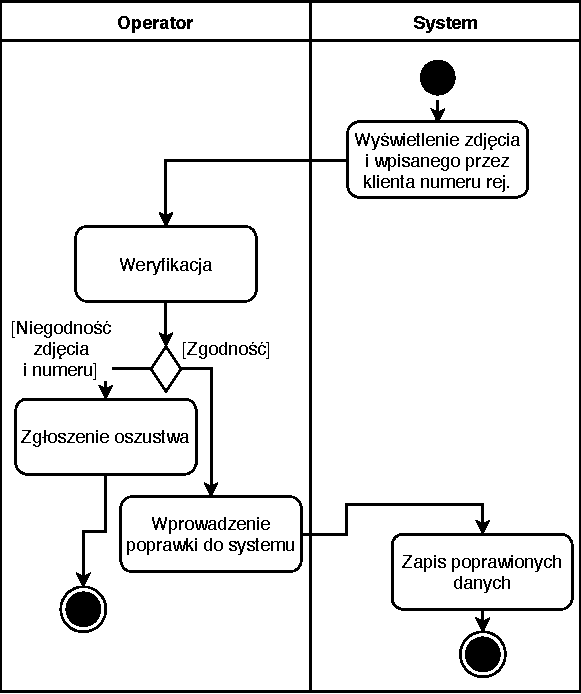
\includegraphics[width=90mm]{diagramy/DiagCzynWyswietlZdjecia.pdf}
	\caption{Diagram czynności: Operator weryfikuje wykryte oszustwo}
\end{figure}

% Diagram czynnosci: Właściciel wyświetla statystyki
\begin{figure}[H]
	\centering
	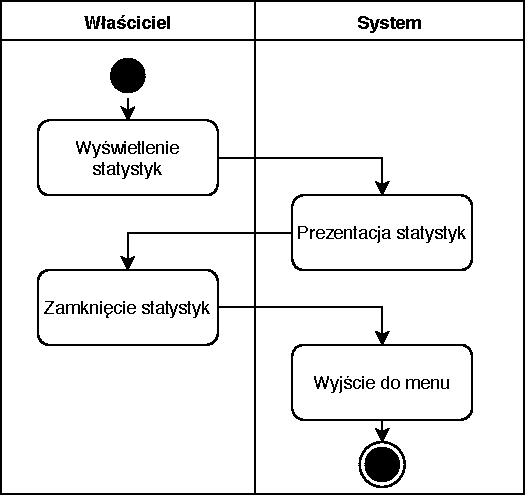
\includegraphics[width=90mm]{diagramy/DiagCzynStatystyki.pdf}
	\caption{Diagram czynności: Właściciel wyświetla statystyki}
\end{figure}




